
\حصہ{تکونیاتی بدل}
ہم \عددی{a^2+x^2}، \عددی{a^2-x^2} اور \عددی{x^2-a^2} میں تکونیاتی بدل پر کر کے  ایک مربع جزو حاصل کرتے ہیں جو ایسے تکمل، جن میں ان کا جذر پایا جاتا ہو، کو سادہ صورت میں بدل دیتا ہے۔ ان سادہ تکمل کا حل نسبتاً آسان  ہوتا ہے۔

\جزوحصہء{تین بنیادی بدل}
تین عمومی بدل \عددی{x=a\tan \theta}، \عددی{x=a\sin\theta} اور \عددی{x=a\sec\theta} ہیں جو شکل \حوالہ{شکل_طریقہ_حوالہ_مثلث} میں قائمہ مثلثوں سے حاصل ہوتے ہیں۔

\عددی{x=a\tan\theta} لیتے ہوئے درج ذیل حاصل ہوتا ہے۔
\begin{align}
a^2+x^2=a^2+a^2\tan^2\theta=a^2(1+\tan^2\theta)=a^2\sec^2\theta
\end{align}

\عددی{x=a\sin\theta} لیتے ہوئے درج ذیل حاصل ہوتا ہے۔
\begin{align}
a^2-x^2=a^2-a^2\sin^2\theta=a^2(1-\sin^2\theta)=a^2\cos^2\theta
\end{align}

\عددی{x=a\sec\theta} لیتے ہوئے درج ذیل حاصل ہوتا ہے۔
\begin{align}
x^2-a^2=a^2\sec^2\theta-a^2=a^2(\sec^2\theta-1)=a^2\tan^2\theta
\end{align}
\موٹا{تکونیاتی بدل}\\
\begin{enumerate}[a.]
\item
\عددی{x=a\tan\theta} لے کر \عددی{a^2+x^2} کی جگہ \عددی{a^2\sec^2\theta} پر کریں۔
\item
\عددی{x=a\sin\theta} لے کر \عددی{a^2-x^2} کی جگہ \عددی{a^2\cos^2\theta} پر کریں۔
\item
\عددی{x=a\sec\theta} لے کر \عددی{x^2-a^2} کی جگہ \عددی{a^2\tan^2\theta} پر کریں۔
\end{enumerate}


\begin{figure}
\centering
\begin{subfigure}{0.3\textwidth}
\centering
\begin{tikzpicture}[font=\small]
\pgfmathsetmacro{\len}{2}
\pgfmathsetmacro{\ang}{30}
\pgfmathsetmacro{\kx}{\len*cos(\ang)}
\pgfmathsetmacro{\ky}{\len*sin(\ang)}
\draw(0,0)--++(\ang:\len)node[pos=0.7,left,yshift=0.5ex]{$\sqrt{a^2+x^2}$}--(\kx,0)node[pos=0.5,right]{$x$}--(0,0)node[pos=0.5,below]{$a$};
\draw([shift={(0:0.5)}]0,0) arc (0:\ang:0.5);
\draw(1/2*\ang:0.7)node[]{$\theta$};
\draw(\x/2,\ky+0.25)node[above]{$\begin{aligned} x&=a\tan\theta\\ \sqrt{a^2+x^2}&=a\abs{\sec\theta} \end{aligned}$};
\end{tikzpicture}
\end{subfigure}\hfill
\begin{subfigure}{0.3\textwidth}
\centering
\begin{tikzpicture}[font=\small]
\pgfmathsetmacro{\len}{2}
\pgfmathsetmacro{\ang}{30}
\pgfmathsetmacro{\kx}{\len*cos(\ang)}
\pgfmathsetmacro{\ky}{\len*sin(\ang)}
\draw(0,0)--++(\ang:\len)node[pos=0.7,left,yshift=0.5ex]{$a$}--(\kx,0)node[pos=0.5,right]{$x$}--(0,0)node[pos=0.5,below]{$\sqrt{a^2-x^2}$};
\draw([shift={(0:0.5)}]0,0) arc (0:\ang:0.5);
\draw(1/2*\ang:0.7)node[]{$\theta$};
\draw(\x/2,\ky+0.25)node[above]{$\begin{aligned} x&=a\sin\theta\\ \sqrt{a^2-x^2}&=a\abs{\cos\theta} \end{aligned}$};
\end{tikzpicture}
\end{subfigure}\hfill
\begin{subfigure}{0.3\textwidth}
\centering
\begin{tikzpicture}[font=\small]
\pgfmathsetmacro{\len}{2}
\pgfmathsetmacro{\ang}{30}
\pgfmathsetmacro{\kx}{\len*cos(\ang)}
\pgfmathsetmacro{\ky}{\len*sin(\ang)}
\draw(0,0)--++(\ang:\len)node[pos=0.7,left,yshift=0.5ex]{$x$}--(\kx,0)node[pos=0.5,right]{$\sqrt{x^2-a^2}$}--(0,0)node[pos=0.5,below]{$a$};
\draw([shift={(0:0.5)}]0,0) arc (0:\ang:0.5);
\draw(1/2*\ang:0.7)node[]{$\theta$};
\draw(\x/2,\ky+0.25)node[above]{$\begin{aligned} x&=a\sec\theta\\ \sqrt{x^2-a^2}&=a\abs{\tan\theta} \end{aligned}$};
\end{tikzpicture}
\end{subfigure}
\caption{تکونیاتی بدل کو حوالہ مثلث۔}
\label{شکل_طریقہ_حوالہ_مثلث}
\end{figure}

ہم ایسا بدل استعمال کرنا چاہیں گے جو قابل واپسی ہو تا کہ آخری قدم پر اس کو واپس کرتے ہوئے اصل متغیرات میں نتیجہ لکھ سکیں۔ مثال کے طور پر اگر \عددی{x=a\tan\theta} کی صورت میں ہم چاہیں گے کہ تکمل لینے کے بعد آخری قدم پر \عددی{\theta=\tan^{-1}\tfrac{x}{a}} لکھنا ممکن ہو۔ اسی طرح \عددی{x=a\sin\theta} کی صورت میں ہم تکمل کے بعد \عددی{\theta=\sin^{-1}\tfrac{x}{a}}  اور \عددی{x=a\sec\theta} کے لئے \عددی{\theta=\sec^{-1}\tfrac{x}{a}} پر کرنا چاہیں گے۔

\begin{figure}
\centering
\begin{subfigure}{0.3\textwidth}
\centering
\begin{tikzpicture}[font=\small,declare function={f(\x)=tan(deg(\x));}]
\pgfmathsetmacro{\k}{pi/2}
\begin{axis}[clip=false,width=4.5cm, axis lines=middle, xlabel={$\tfrac{x}{a}$},ylabel={$\theta$},xlabel style={at={(current axis.right of origin)},anchor=west},ylabel style={at={(current axis.above origin)},anchor=south},xtick={\empty},ytick={-\k,\k},yticklabels={$-\tfrac{\pi}{2}$,$\tfrac{\pi}{2}$},enlargelimits={0.2}]
\addplot[domain=-\k+0.2:\k-0.2]({f(x)},x);
\draw({f(-\k+0.2)},-\k)--({f(\k-0.2)},-\k);
\draw({f(-\k+0.2)},\k)--({f(\k-0.2)},\k);
\draw(0,{1/2*\k})node[left]{$\theta=\tan^{-1}\frac{x}{a}$};
\end{axis}
\end{tikzpicture}
\end{subfigure}\hfill
\begin{subfigure}{0.3\textwidth}
\centering
\begin{tikzpicture}[font=\small,declare function={f(\x)=sin(deg(\x));}]
\pgfmathsetmacro{\k}{pi/2}
\begin{axis}[clip=false,width=4.5cm, axis lines=middle, xlabel={$\tfrac{x}{a}$},ylabel={$\theta$},xlabel style={at={(current axis.right of origin)},anchor=west},ylabel style={at={(current axis.above origin)},anchor=south},xtick={-1,1},ytick={-\k,\k},yticklabels={$-\tfrac{\pi}{2}$,$\tfrac{\pi}{2}$},enlargelimits={0.2}]
\addplot[domain=-\k+0.2:\k-0.2]({f(x)},x);
\draw(0,{1/2*\k})node[left]{$\theta=\sin^{-1}\frac{x}{a}$};
\end{axis}
\end{tikzpicture}
\end{subfigure}\hfill
\begin{subfigure}{0.3\textwidth}
\centering
\begin{tikzpicture}[font=\small,declare function={f(\x)=sec(deg(\x));}]
\pgfmathsetmacro{\k}{pi/2}
\pgfmathsetmacro{\kk}{pi}
\begin{axis}[clip=false,width=4.5cm, axis lines=middle, xlabel={$\tfrac{x}{a}$},ylabel={$\theta$},xlabel style={at={(current axis.right of origin)},anchor=west},ylabel style={at={(current axis.above origin)},anchor=south},xtick={-1,1},ytick={\k,\kk},yticklabels={$\tfrac{\pi}{2}$,$\pi$},enlargelimits={0.2}]
\addplot[domain=0:\k-0.4]({f(x)},x);
\addplot[domain=\k+0.4:2*\k]({f(x)},x);
\draw({f(\k+0.4)},\k)--({f(\k-0.4)},\k);
\draw(0,{6/4*\k})node[right]{$\theta=\sec^{-1}\frac{x}{a}$};
\end{axis}
\end{tikzpicture}
\end{subfigure}
\caption{الٹ تکونیاتی تفاعل کے ترسیمات۔}
\label{شکل_طریقے_الٹ_کے_وقفے}
\end{figure}
جیسا ہم حصہ \حوالہ{حصہ_ماورائی_الٹ_تکونیاتی_تفاعل} سے جانتے ہیں ان تفاعل کے الٹ صرف مخصوص وقفہ پر پائے جاتے ہیں (شکل \حوالہ{شکل_طریقے_الٹ_کے_وقفے})۔ الٹ کے لئے درج ذیل ضروری ہے۔
\begin{enumerate}[a.]
\item
\عددی{x=a\tan\theta} کا الٹ \عددی{\theta=\tan^{-1}\tfrac{x}{a}} وقفہ \عددی{-\frac{\pi}{2}<\theta<\frac{\pi}{2}} پر ہو گا۔ 
\item
\عددی{x=a\sin\theta} کا الٹ \عددی{\theta=\sin^{-1}\tfrac{x}{a}} وقفہ \عددی{-\frac{\pi}{2}<\theta<\frac{\pi}{2}} پر ہو گا۔ 
\item
\عددی{x=a\sec\theta} کا الٹ \عددی{\theta=\sec^{-1}\tfrac{x}{a}} وقفہ
 \عددی{0\le \theta<\frac{\pi}{2}} پر  \عددی{\frac{x}{a}\ge 1} کی صورت میں  اور وقفہ \عددی{\tfrac{\pi}{2}<\theta\le \pi} پر \عددی{\tfrac{x}{a}\le -1} کی صورت میں  ہو گا۔ 
\end{enumerate}

حساب کتاب آسان بنانے کی خاطر ہم  بدل \عددی{x=a\sec\theta} کے استعمال کو ان تکمل تک پابند کرتے ہیں جن میں   \عددی{\tfrac{x}{a}\ge 1} ہو۔اس طرح  \عددی{\theta} وقفہ \عددی{[0,\tfrac{\pi}{2})} میں ہو گا جہاں \عددی{\tan\theta\ge 0} ہو گا۔ یوں \عددی{a>0} کی صورت میں 
\begin{align*}
\sqrt{x^2-a^2}=\sqrt{a^2\tan^2\theta}=\abs{a\tan\theta}=a\tan\theta
\end{align*}
 ہو گا جو مطلق کی علامت سے آزاد ہے۔


\ابتدا{مثال}\شناخت{مثال_طریقہ_حوالہ_مثلث_الف}
تکمل \عددی{\int\tfrac{\dif x}{\sqrt{4+x^2}}} حل کریں۔

حل:\quad
ہم درج ذیل لیتے ہیں۔
\begin{align*}
x=2\tan\theta,\quad \dif x=2\sec^2\theta\dif\theta,\quad -\frac{\pi}{2}<\theta<\frac{\pi}{2}\\
4+x^2=4+4\tan^2\theta=4(1+\tan^2\theta)=4\sec^2\theta
\end{align*}
یوں
\begin{align*}
\int\frac{\dif x}{\sqrt{4+x^2}}&=\int \frac{2\sec^2\theta\dif\theta}{\sqrt{4\sec^2\theta}}=\int\frac{\sec^2\theta\dif \theta}{\abs{\sec\theta}}&& \sqrt{\sec^2\theta}=\abs{\sec\theta}\\
&=\int \sec\theta\dif \theta\\
&=\ln\abs{\sec\theta+\tan\theta}+C\\
&=\ln\abs{\frac{\sqrt{4+x^2}}{2}+\frac{x}{2}}+C&&\text{\RL{شکل \حوالہ{شکل_مثال_طریقہ_حوالہ_مثلث_الف}}}\\
&=\ln\abs{\sqrt{4+x^2}+x}+C'&&C'=C-\ln 2
\end{align*}
ہو گا۔ آپ اس پر دوبارہ نظر ڈالیں کہ ہم نے \عددی{\ln\abs{\sec\theta+\tan\theta}} کو \عددی{x} کی صورت میں کس طرح لکھا۔ ہم نے ابتدائی بدل \عددی{x=2\tan\theta} کے لئے حوالہ مثلث (شکل \حوالہ{شکل_مثال_طریقہ_حوالہ_مثلث_الف}) کا خاکہ بنایا اور اسی سے نسبتیں \عددی{\tan\theta=\tfrac{x}{2}} اور \عددی{\sec\theta=\tfrac{\sqrt{4+x^2}}{2}} پڑھیں۔
\انتہا{مثال}
%======================
\begin{figure}
\centering
\begin{minipage}{0.30\textwidth}
\centering
\begin{tikzpicture}
\pgfmathsetmacro{\r}{2}
\pgfmathsetmacro{\ang}{30}
\draw(0,0)--++(\ang:\r)coordinate(ka)node[pos=0.7,left,yshift=0.5ex]{$\sqrt{4+x^2}$}--($(0,0)!(ka)!(2,0)$)node[pos=0.5,right]{$x$}--(0,0)node[pos=0.5,below]{$2$};
\draw([shift={(0:0.5)}]0,0) arc (0:\ang:0.5);
\draw(1/2*\ang:0.7)node[]{$\theta$};
\end{tikzpicture}
\caption{حوالہ مثلث برائے مثال \حوالہ{مثال_طریقہ_حوالہ_مثلث_الف}}
\label{شکل_مثال_طریقہ_حوالہ_مثلث_الف}
\end{minipage}\hfill
\begin{minipage}{0.30\textwidth}
\centering
\begin{tikzpicture}
\pgfmathsetmacro{\r}{2}
\pgfmathsetmacro{\ang}{30}
\draw(0,0)--++(\ang:\r)coordinate(ka)node[pos=0.7,left,yshift=0.5ex]{$3$}--($(0,0)!(ka)!(2,0)$)node[pos=0.5,right]{$x$}--(0,0)node[pos=0.5,below]{$\sqrt{9-x^2}$};
\draw([shift={(0:0.5)}]0,0) arc (0:\ang:0.5);
\draw(1/2*\ang:0.7)node[]{$\theta$};
\end{tikzpicture}
\caption{حوالہ مثلث برائے مثال \حوالہ{مثال_طریقہ_حوالہ_مثلث_ب}}
\label{شکل_مثال_طریقہ_حوالہ_مثلث_ب}
\end{minipage}\hfill
\begin{minipage}{0.30\textwidth}
\centering
\begin{tikzpicture}
\pgfmathsetmacro{\r}{2}
\pgfmathsetmacro{\ang}{30}
\draw(0,0)--++(\ang:\r)coordinate(ka)node[pos=0.7,left,yshift=0.5ex]{$5x$}--($(0,0)!(ka)!(2,0)$)node[pos=0.5,right]{$\sqrt{25x^2-4}$}--(0,0)node[pos=0.5,below]{$2$};
\draw([shift={(0:0.5)}]0,0) arc (0:\ang:0.5);
\draw(1/2*\ang:0.7)node[]{$\theta$};
\end{tikzpicture}
\caption{حوالہ مثلث برائے مثال \حوالہ{مثال_طریقہ_حوالہ_مثلث_پ}}
\label{شکل_مثال_طریقہ_حوالہ_مثلث_پ}
\end{minipage}
\end{figure}

\ابتدا{مثال}\شناخت{مثال_طریقہ_حوالہ_مثلث_ب}
تکمل \عددی{\int\tfrac{x^2\dif x}{\sqrt{9-x^2}}} حل کریں۔

حل:\quad
جزو \عددی{9-x^2} کی جگہ ایک مربع جزو پر کرنے کی خاطر ہم درج ذیل لیتے ہیں۔
\begin{align*}
x=3\sin\theta,\quad &\dif x=3\cos\theta\dif\theta,\quad -\frac{\pi}{2}<\theta<\frac{\pi}{2}\\
9-x^2&=9(1-\sin^2\theta)=9\cos^2\theta
\end{align*}
یوں
\begin{align*}
\int\frac{x^2\dif x}{\sqrt{9-x^2}}&=\int\frac{9\sin^2\theta\cdot3\cos\theta\dif\theta}{\abs{3\cos\theta}}\\
&=9\int \sin^2\theta\dif \theta\\
&=9\int \frac{1-\cos2\theta}{2}\dif\theta\\
&=\frac{9}{2}\big(\theta-\frac{\sin2\theta}{2}\big)+C\\
&=\frac{9}{2}(\theta-\sin\theta\cos\theta)+C\\
&=\frac{9}{2}\big(\sin^{-1}\frac{x}{3}-\frac{x}{3}\cdot\frac{\sqrt{9-x^2}}{3}\big)+C&&\text{\RL{شکل \حوالہ{شکل_مثال_طریقہ_حوالہ_مثلث_ب}}}\\
&=\frac{9}{2}\sin^{-1}\frac{x}{3}-\frac{x}{2}\sqrt{9-x^2}+C
\end{align*}
ہو گا جہاں شکل \حوالہ{شکل_مثال_طریقہ_حوالہ_مثلث_ب} سے نسبتیں \عددی{\sin\theta=\tfrac{x}{3}} اور \عددی{\cos\theta=\tfrac{\sqrt{9-x^2}}{3}} پڑھی گئی ہیں۔
\انتہا{مثال}
%===============
\ابتدا{مثال}\شناخت{مثال_طریقہ_حوالہ_مثلث_پ}
تکمل \عددی{\int\tfrac{\dif x}{\sqrt{25x^2-4}},\, x>\tfrac{2}{5}} حل کریں۔

حل:\quad
ہم جذر کو
\begin{align*}
\sqrt{25x^2-4}=\sqrt{25\big(x^2-\frac{4}{25}\big)}=5\sqrt{x^2-\big(\tfrac{2}{5}\big)^2}
\end{align*}
صورت میں لکھتے ہیں تا کہ یہ \عددی{x^2-a^2} روپ میں ہو۔ اس کے بعد درج ذیل بدل استعمال کرتے ہیں۔
\begin{align*}
x&=\frac{2}{5}\sec\theta,\quad \dif x=\frac{2}{5}\sec\theta\tan\theta\dif\theta,\quad 0<\theta<\frac{\pi}{2}\\
x^2-\big(\frac{2}{5}\big)^2&=\frac{4}{25}\sec^2\theta-\frac{4}{25}=\frac{4}{25}(\sec^2\theta-1)=\frac{4}{25}\tan^2\theta\\
\sqrt{x^2-\big(\frac{2}{5}\big)^2}&=\frac{2}{5}\abs{\tan \theta}=\frac{2}{5}\tan\theta&&\tan\theta>0,\, 0<\theta<\frac{\pi}{2}
\end{align*}
یوں
\begin{align*}
\int\frac{\dif x}{\sqrt{25x^2-4}}&=\int\frac{\dif x}{5\sqrt{x^2-(4/25)}}=\int\frac{(2/5)\sec\theta\tan\theta\dif\theta}{5\cdot(2/5)\tan\theta}\\
&=\frac{1}{5}\int \sec\theta\dif\theta=\frac{1}{5}\ln\abs{\sec\theta+\tan\theta}+C\\
&=\frac{1}{5}\ln\abs{\frac{5x}{2}+\frac{\sqrt{25x^2-4}}{2}}+C
\end{align*}
ہو گا جہاں تکونیاتی نسبت شکل \حوالہ{مثال_طریقہ_حوالہ_مثلث_پ} سے پڑھی گئی ہے۔ 
\انتہا{مثال}
%=======================
بعض اوقات دو درجی جزو کے طاقت کا تکمل تکونیاتی بدل سے ممکن ہوتا ہے۔ آئیں اگلی مثال میں اس عمل کو دیکھیں۔

\ابتدا{مثال}
منحنی \عددی{y=\tfrac{4}{x^2+4}}، محور \عددی{x}، لکیر \عددی{x=0} اور \عددی{x=2} کے بیچ خطہ کو محور \عددی{x} کے گرد گھما کر جسم طواف پیدا کیا جاتا ہے۔ اس جسم کا حجم تلاش کریں۔

حل:\quad
ہم اس خطہ کو ترسیم کر کے ترکیب قرص (حصہ \حوالہ{حصہ_استعمال_تکمل_قرص_اور_چھلا}) سے حجم تلاش کرتے ہیں۔
\begin{align*}
H&=\int_0^2\pi[R(x)]^2\dif x=16\pi\int_0^2\frac{\dif x}{(x^2+4)^2}&&R(x)=\frac{4}{x^2+4}
\end{align*}
اس تکمل کو حل کرنے کی خاطر ہم درج ذیل لیتے ہیں۔
\begin{align*}
x&=2\tan\theta,\quad \dif x=2\sec^2\theta\dif\theta,\quad \theta=\tan^{-1}\frac{x}{2}\\
x^2+4&=4\tan^2\theta+4,\quad 4(\tan^2\theta+1)=4\sec^2\theta 
\end{align*}
یوں درج ذیل حاصل ہو گا۔
\begin{align*}
H&=16\pi\int_0^2\frac{\dif x}{(x^2+4)^2}\\
&=16\pi\int_0^{\pi/4}\frac{2\sec^2\theta\dif\theta}{(4\sec^2\theta)^2}\\
&=16\pi\int_0^{\pi/4}\frac{2\sec^2\theta\dif\theta}{16\sec^4\theta}=\pi\int_0^{\pi/4}2\cos^2\theta\dif\theta\\
&=\pi\int_0^{\pi/4}(1+\cos 2\theta)\dif \theta=\pi\left[\theta+\frac{\sin2\theta}{2}\right]_0^{\pi/4}\\
&=\pi\big[\frac{\pi}{4}+\frac{1}{2}\big]\approx 4.04
\end{align*}
\انتہا{مثال}
%=================

\حصہء{سوالات}

